\chapter{Respirazione e apparato respiratorio}
\label{capitolo:preliminari:respirazione}

\section{Anatomia dell'apparato respiratorio}

L'\emph{apparato respiratorio} (o anche sistema respiratorio) \`e un sistema biologico atto alla respirazione. Negli esseri umani l'anatomia funzionale dell'apparato respiratorio include \cite{anatomiaRespiratorio}:

\begin{figure}
 \centering
 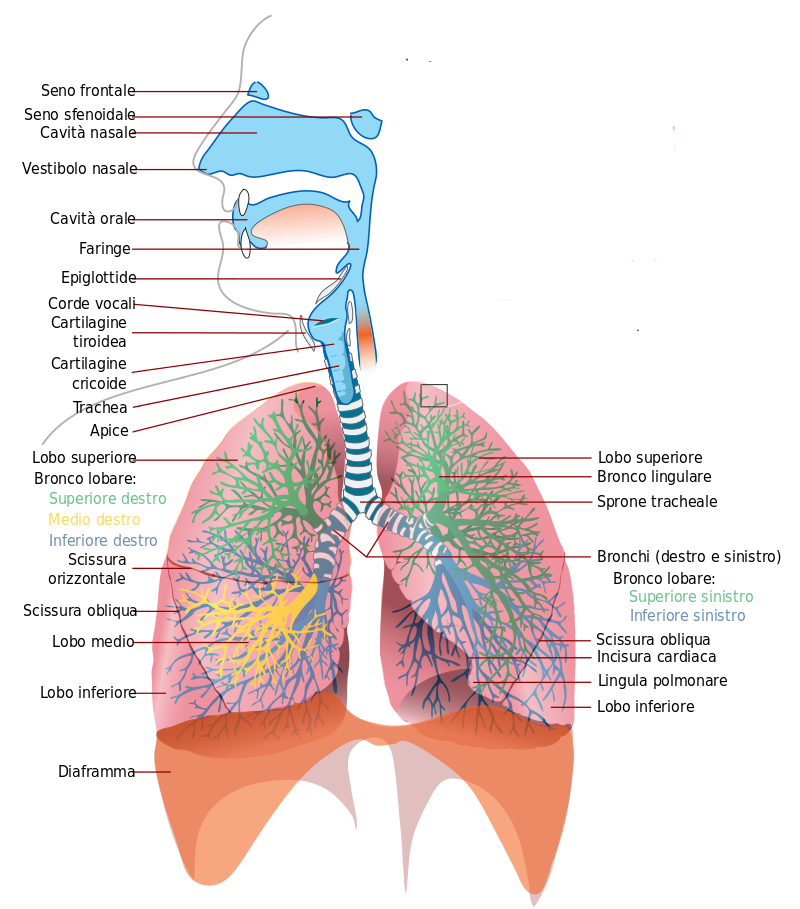
\includegraphics[width=0.6\textwidth]{./Respiratory_system_complete_it.png}
 % appaRespi.jpg: 571x483 pixel, 72dpi, 20.14x17.04 cm, bb=0 0 571 483
  \label{apparatoRespiratorio}
\end{figure}



% \begin{description}
%   \item[Vie aeree.]
\begin{bf}Vie aeree.\end{bf}
    Le vie aeree sono cavit\`a in cui le sostanze gassose, vengono trasportate da o verso i polmoni. Le seguenti parti del corpo sono vie aeree: naso esterno, cavit\`a orale, faringe, laringe, trachea. La figura \ref{apparatoRespiratorio} \cite{appaRespi} \`e una rappresentazione pi\`u esaustiva dell'apparato respiratorio.
%   \item[Polmoni.]


\begin{bf}Polmoni.\end{bf}
    I polmoni sono l'organo essenziale per la respirazione. 
    La loro principale funzione \`e quella di trasportare l'ossigeno dell'ambiente circostante al sangue e di espellere l'anidride carbonica. 
    I polmoni contengono delle piccole sacche d'aria chiamate alveoli. 
    Attraverso i capillari degli alveoli avviene lo scambio per diffusione di ossigeno ed anidride carbonica tra il sangue dell'organismo e l'aria contenuta negli alveoli. 
    Il polmone destro \`e diviso in tre lobi: superiore, medio ed inferiore; mentre quello polmone sinistro \`e diviso in due lobi: uno superiore ed uno inferiore. 
%   \item[Muscoli respiratori.]


\begin{bf}Muscoli respiratori.\end{bf}
    I muscoli respiratori sono il diaframma, i muscoli intercostali, i muscoli addominali, lo sternocleidomastoideo e i muscoli scaleni. Questi muscoli causano l'espansione polmonare.
% \end{description}




\section{Respirazione}

La \emph{respirazione} \`e il processo attraverso il quale l'organismo scambia aria tra i polmoni e l'ambiente circostante. 
La respirazione permette di acquisire ossigeno nel sangue che viene poi usato nel metabolismo e permette di eliminare i residui gassosi del metabolismo come l'anidride carbonica. Durante la respirazione si scambia anche vapore acqueo. 
Il termine usato per indicare il respiro in condizioni normali \`e \emph{eupnea}.  

\subsection{Meccanica della respirazione}

La respirazione \`e ciclica e un ciclo di respirazione ha atto in tre fasi consecutive \cite{meccanicaRespi, wikiMeccaRespi}:
\begin{description}
  \item[Inspirazione.]
    Durante questa fase l'aria viene introdotta nei polmoni. L'inspirazione avviene grazie alla contrazione dei muscoli intercostali e del diaframma, tale contrazione provoca un aumento di volume polmonare e una diminuzione della pressione intrapleurica: ne consegue un'aspirazione dell'aria nei polmoni.
  \item[Espirazione.]
    Durante questa fase l'aria viene espulsa dai polmoni. 
    \`E determinata dal rilascio della forza elastica del parenchima polmonare. Il volume toracico diminuisce, i polmoni vengono compressi e l'aria espulsa.
    \item[Pausa.]
    Tra una espirazione e l'inspirazione successiva ci pu\`o essere una pausa di durata variabile. 
\end{description}

\section{Diagnosi delle malattie dell'apparato respiratorio}



\subsection{Spirometro con pneumotacografo}
Lo spirometro \`e uno strumento utilizzato per misurare i volumi d'aria polmonari. \`E composto da un sensore collegato a un boccaglio, attraverso il quale il paziente respira e da una parte che misura i movimenti di aria provocati dal soggetto. 
Lo spirometro con pneumotacografo \`e un tipo di spirometro dotato di una lamina con la funzione di restringimento e che causa una differenza di pressione. 
Questa differenza pressoria viene misurata da un manometro e poi riconvertita in un segnale proporzionale al flusso generato \cite{WikiSpirPneu, PneumotacofragoTreCani}.

\subsection{Polissonnografia}
La \emph{polisonnografia} \`e una tecnica diagnostica che consiste nella registrazione simultanea di pi\`u parametri fisiologici durante la notte. Normalmente nel corso del test vengono registrati: il flusso d'aria della respirazione, il livello di ossigeno nel sangue, la posizione del corpo, l'attivit\`a cerebrale (attraverso un elettroencefalografo), il movimento degli occhi (attraverso un elettrooculografo) e l'attivit\`a cardiaca (attraverso un elettrocardiografo) \cite{polisonnografo}.

\subsection{Auscultazione}
L'\emph{auscultazione} \`e un sistema di diagnosi che consiste nell'ascoltare i suoni interni del corpo.
Nella accezione che ci interessa, il termine auscultazione ha il significato di ascoltare attraverso uno stetoscopio i suoni prodotti dall'apparato respiratorio. Lo stetoscopio pu\`o essere posizionato in varie parti del torace e della schiena \cite{CARPDWAM}. 

\subsection{Stetoscopio}

Lo stetoscopio
% (dal greco στήθος, stéthos petto, e σκοπή, skopé osservazione) 
\`e uno strumento medico utile all'auscultazione delle parti interne del corpo e sopratutto del torace. Ci sono due tipi principali di stetoscopio:
\paragraph{Stetoscopio acustico.}
    Lo stetoscopio acustico funziona tramite la trasmissione di suoni provenienti dal corpo attraverso dei canali contenenti aria fino alle orecchie dell'ascoltatore.
    Uno dei problemi degli stetoscopi acustici \`e il basso volume del suono trasmesso. 
    Ne consegue una difficolt\`a nell'eseguire una diagnosi precisa.
\paragraph{Stetoscopio elettronico.}
    L'innovazione tecnologica nel campo degli stetoscopi consente oggi la rilevazione di una pi\`u ampia gamma di suoni ed una maggior qualit\`a d'ascolto, con la possibilit\`a di ottenere registrazioni e riproduzioni di grande fedelt\`a dei suoni. 
    A differenza degli stetoscopi acustici, che sono tutti basati sullo stesso metodo di funzionamento, gli stetoscopi elettronici variano molto tra un modello e l'altro. 
    I pi\`u semplici funzionano grazie ad un microfono applicato al petto del paziente, ma di contro, risentono del suono dell'ambiente esterno che spesso causa interferenze. 
    Alcuni stetoscopi elettronici forniscono direttamente un audio in output e si possono usare insieme ad un dispositivo esterno di registrazione. 
    Altri possono trasmettere il segnale via wireless o bluethoot. Un dispositivo (ad esempio un computer) riceve questo segnale e pu\`o fare vari tipi di analisi. 
    Altri modelli, pi\`u complessi, trasformano le onde sonore in impulsi elettrici, cos\`i da poter essere amplificate per un migliore ascolto. 
    Recentemente, alcuni stetoscopi elettronici sono stati dotati di filtri, allo scopo di eliminare le interferenze sonore esterne e in pi\`u sono in grado di poter selezionare il range di frequenza in modo da poter ascoltare separatamente o meno i suoni cardiaci da quelli respiratori. \cite{fusello}


\subsection{Invasivit\`a clinica}

Un parametro molto importante per valutare un sistema diagnostico \`e l'invasivit\`a clinica o semplicemente invasivit\`a. 
Questa si riferisce alla possibilit\`a che l'esame finisca per compromettere ulteriormente lo stato di salute del soggetto. 
Siamo in presenza di un esame invasivo ad esempio, nel caso in cui l'esame possa portare agenti contaminanti (virus, batteri, tossine, sporcizia) all'interno del diretto interessato e quindi causare una infezione che aggravi le condizioni del paziente. 
L'invasivit\`a di un meccanismo diagnostico esce allo scoperto anche nei casi in cui un piccolo errore nella procedura procura danni al paziente \cite{Invasivita}.
Tra i sistemi diagnostici descritti in questa sezione il metodo meno invasivo \`e l'auscultazione.


\section{Patologia dell'apparato respiratorio}

\subsection{Apnee del sonno}
La \emph{sindrome da apnea del sonno} \`e un disordine del sonno caratterizzato da ripetute apnee o ipopnee durante il sonno \cite{ASDBOS}. 
Una \emph{apnea} \`e una pausa di durata anormale nella respirazione che supera i dieci secondi \cite{OSARFSD} e pu\`o durare anche alcuni minuti \cite{NHLBI}. 
Una \emph{ipopnea} \`e un evento caratterizzato da respirazione insufficiente, pi\`u precisamente una ipopnea si verifica quando il flusso d'aria si riduce di almeno il $30\%$ per almeno dieci secondi e la desaturazione di ossigeno nel sangue \`e di almeno il $4\%$ \cite{OSARFSD}. 
Ci sono tre forme di apnea del sonno:
\begin{description}
  \item[Apnea centrale.]
   La respirazione \`e interrotta per via di un mancato movimento dei muscoli respiratori, quindi il volume dei polmoni rimane invariato.
  \item[Apnea ostruttiva.]
    La respirazione \`e interrotta a causa di un blocco fisico nelle vie aeree nonostante persistano movimenti respiratori \cite{AntoniettaBisulli}.
  \item[Apnea mista.]
    La respirazione \`e soggetta a entrambi i tipi di apnea appena descritti.
\end{description}

Le apnee del sonno si verificano sia nei bambini che negli adulti. I soggetti affetti da apnea del sonno possono manifestare i seguenti sintomi: eccessiva sonnolenza durante il giorno, tempi di reazione lenti, problemi alla vista, indebolimento delle funzioni del fegato e altro. 
Inoltre gravi forme di apnee del sonno ostruttive aumentano in modo significativo il rischio di eventi cardiovascolari fatali \cite{OSARFSD, ASAHAIS, SSAAROISITE}.

L'\emph{indice di apnea-ipopnea(apnea-hypopnea index AHI)} \`e definito come il numero di eventi di apnea e di ipopnea in rapporto alla durata del sonno. 
L'AHI \`e un indicatore della gravit\`a della sindrome di apnea del sonno e i suoi valori sono categorizzati tipicamente in: leggera da 5 a 15 episodi all'ora, moderata da 15 a 30 episodi all'ora o severa oltre i 30 episodi all'ora. 

Lo studio \cite{ASDBOS} conclude che c'\`e una forte associazione tra la sindrome da apnea del sonno e l'ictus. 
In particolare dimostra che un indice da moderato a severo di AHI \`e associato ad un alto rischio di ictus e ipotizza che la sindrome da apnea del sonno contribuisca allo sviluppo di un ictus. 
Purtroppo resta ancora da scoprire se esiste un pattern respiratorio specifico che precede immediatamente un ictus.

Lo studio \cite{DNPSDOSA} prende in esame i polisonnogrammi e i certificati di morte di alcune persone che sono decedute a causa di una malattia cardiaca improvvisa. 
Le persone sono state divise in due gruppi: le persone del primo gruppo soffrivano di sindrome da apnea notturna mentre le persone del secondo no. 
Si \`e riscontrato che la maggior parte delle persone appartenenti al primo gruppo sono morte durante il sonno al contrario di quelle del secondo. 
Lo studio conclude che la gravit\`a della sindrome da apnea del sonno \`e direttamente proporzionale al rischio di morte improvvisa per malattie cardiache durante il sonno. 
\\Episodi acuti di apnea o ipopnea possono indurre: ipossiemia, aumento degli impulsi nel sistema nervoso simpatico, aumento brusco nella pressione sanguigna, aumento dello stress delle pareti cardiache, aritmie cardiache, ipercoagulabilit\`a, stress ossidativo vascolare, infiammazioni sistemiche e altro. 
Questo potrebbe spiegare i dati osservati dallo studio. Resta un problema aperto quello di stabilire se nel primo gruppo di persone, la morte \`e immediatamente preceduta da un evento di apnea o ipopnea grave. 


\subsection{Arresto respiratorio}
Un arresto respiratorio \`e l'interruzione della respirazione normale. \`E molto probabile che si verifichino traumi celebrali se l'arresto respiratorio dura pi\`u di tre minuti e la morte \`e quasi certa se questo dura pi\`u di cinque minuti.

\section{Base funzionale dei suoni respiratori}

Secondo \cite{PKW} i suoni normali che si possono sentire sul petto di un soggetto nella fase di inspirazione, vengono generati sopratutto nella parte lobare delle vie respiratorie. I suoni respiratori sono generati da turbolenze dell'aria nelle vie respiratorie. Le caratteristiche dei suoni sono molto variabili, si possono notare differenze da persona a persona che dipendono dal peso, dall'et\`a, dallo stato di salute e altri fattori. I suoni respiratori variano anche rispetto alla densit\`a del gas respirato la quale diminuisce con l'aumentare dell'altitudine rispetto al livello del mare. In generale per\`o l'intensit\`a dei suoni respiratori \`e proporzionale al quadrato del flusso d'aria. 
% mentre nella fase di espirazione questi vengono sopratutto da regioni pi\`u vicine.
Lo studio \cite{DOIAERSINTSOTHT} nota che i suoni inspiratori vengono prodotti in modo predominante nella zone periferiche dei polmoni, mentre i suoni espiratori vengono prodotti nelle zone pi\`u centrali.

\section{Analisi acustica dei suoni respiratori}
\label{sec:Analisiacusticadeisuonirespiratori}

L'articolo \cite{GPA} analizza l'energia spettrale dei suoni respiratori normali ascoltati sul petto di un soggetto. Conclude che questi seguono uno schema caratteristico, in particolare che la potenza decresce in modo esponenziale con la frequenza nell'intervallo dai $75$ ai $2000 Hz$, dopo quest'ultimo valore la potenza \`e trascurabile. Secondo \cite{SKCAKM} il suono registrato sul petto di soggetti sani ha una intensit\`a massima attorno ai $250Hz$ e decresce rapidamente fino ad arrivare ad un livello di intensit\`a trascurabile attorno a una frequenza di circa $1000Hz$. Nel caso dei soggetti malati invece i picchi di frequenze sono pi\`u alti.


Gli articoli \cite{ADT, KoronaKokar, kandaswamy, CACMVS} classificano i suoni respiratori nel modo seguente (riassunto nella figura \ref{classificazioneRespiratori}):
\subparagraph{Suoni respiratori normali}
    I suoni respiratori normali o fisiologici sono i suoni prodotti dal sistema respiratorio di un soggetto sano. 
    Questi suoni sono pi\`u intensi in fase inspiratoria e decrescono in fase espiratoria (nonostante quest'ultima sia pi\`u lunga di quella inspiratoria) e ci\`o \`e dovuto al fatto che l'inspirazione avviene mediante contrazione muscolare, generando un flusso d'aria pi\`u veloce, rispetto all'espirazione, che \`e un fenomeno passivo. 
    I suoni normali hanno un frequenza nell'intervallo dai $100$ ai $1000Hz$. 
    A causa dei suoni prodotti dal movimento dei muscoli del torace e dal diaframma e a causa di quelli prodotti dall'apparato cardiocircolatorio, i suoni dall'apparato respiratorio di solito non vengono studiati a frequenze minori di $60Hz$. 
    I suoni respiratori normali si dividono in:
    \begin{description}
      \item[Murmori vescicolari]
	Si generano per l'azione di filtro degli alveoli sull'aria in arrivo.
      \item[Suoni bronchiali]
	Si generano nelle zone di passaggio dall'albero bronchiale agli alveoli, quindi per mescolanza di rumore bronchiale ed alveolare. 
      \item[Soffio bronchiale]
	Si ascolta in corrispondenza dei grossi bronchi in presenza di addensamento polmonare.
    \end{description}
    
\subparagraph{Suoni respiratori anormali}
    I suoni respiratori anormali o patologici, sono suoni accidentali che non fanno parte del normale ciclo di respirazione. 
    Ci sono due tipi di suoni anormali:
    \begin{description}
      \item[Continui]
	Tra i suoni anormali continui si distinguono: 
	\begin{description}
	  \item[Ronchi o gemiti]
	    Questi suoni sono spesso gravi e sembrano dei rantoli, la loro frequenza dominante \`e $200Hz$, hanno quindi una bassa tonalit\`a. 
	    Sono segno di broncocostrizione e si generano per il passaggio dell'aria in vie aeree ristrette per la presenza di muco o broncospasmo.
	  \item[Rantolo secco (wheezes)]
	    Questi suoni hanno una frequenza dominante attorno ai $100Hz$ e hanno una durata maggiore di $100ms$. 
	    Sono un segnale caratteristico di una malattia ostruttiva polmonare.
	  \item[Sibili]
	    Questi suoni sono dei $wheezes$ molto pi\`u forti e sono la conseguenza di una ostruzione dinamica nella laringe o nella trachea. 
	    L'energia di questi suoni \`e concentrata in massima parte su una frequenza che si aggira attorno ai $1000Hz$.
	\end{description}
      \item[Discontinui]
	Tra i suoni anormali discontinui si notano:
	\begin{description}
	  \item[Rantolo (Crackles)]
	    Questi suoni hanno una durata minore di $10ms$ e cadono in un vasto spettro di frequenze, tra $200$ e $2000Hz$. Di solito sono indice di malattie cardiorespiratorie.
	  \item[Fine  crackles]
	    Sono i rantoli fini, anche detti rantoli crepitanti e hanno una tonalit\`a alta. Sono dovuti alla ritardata apertura degli alveoli. Talvolta ad essi si sovrappongono gli sfregamenti pleurici, il cui reperto \`e molto simile.
	  \item[Coarse crackles]
	    Sono i rantoli subcrepitanti, di una tonalit\`a bassa, il cui reperto si modifica con la tosse. Sono segno di bronchite e si generano per il passaggio dell'aria attraverso il muco.
	  \item[Squawks]
	    Questi suoni sono dei sibili di breve durata.
	\end{description}
    \end{description}


% 
% \begin{table} [h]
%   \begin{tabular}{l l l l}
%     Suono			& Durata 		& Spettro   		  	& Tipo\\
%     \hline\\	
%     suoni normali bronchiali   & -	 		& da $100Hz$ a $1000Hz$		& normale continuo\\
%     suoni normali vescicolari  & -			& da $100Hz$ a $1000Hz$		& normale continuo\\
%     ronchi			& -			& $\sim 200Hz$			& anormale continuo\\
%     wheeze	 		&da $100ms$ a $250ms$	& $\sim 100Hz$			& anormale continuo\\
%     stridor			&-			& $\sim 1000Hz$			& anormale continuo\\
%     crackles			&$<10ms$		&da $200$ a $2000Hz$		& anormale discontinuo\\
%     squawks 			&			&				& anormalediscontinuo\\
%     \hline\\
%   \end{tabular}
% \caption{Classificazione dei suoni respiratori}
% \label{ClassificazioneSuoniRespiratori}
% \end{table}



\begin{center}
\begin{figure}
 

\begin{tikzpicture}
%   [scale=.8,auto=left,every node/.style={fill=blue!20}]
[->,>=stealth',shorten >=1pt,auto,node distance=3cm,
  thick,main node/.style={circle,fill=blue!20,draw,font=\sffamily\Large\bfseries}]
  \node (respiri) at 	(0,3) {suoni respiratori};

  \node (normali) at 	(3,2) {normali};
  \node (anormali) at 	(3,4) {anormali};

  \node (vescicolari) at 	(7,2) {vescicolari};
  \node (bronchiali) at 	(7,1) {bronchiali};
  \node (soffi) at 		(7,1.5) {soffi};

  \node (continui) at 		(7,3) {continui};
  \node (discontinui) at 	(7,5) {discontinui};

  \node (ronchi) at 		(11,2.5) {ronchi};
  \node (rantoli) at 		(11,3) {rantoli};
  \node (sibili) at 		(11,3.5) {sibili};

  \node (fine) at 		(11,4.5) {fine crackles};
  \node (squawks) at 		(11,5) {squawks};
  \node (coarse) at 		(11,5.5) {coarse crackles};  


   \foreach \from/\to in {respiri/normali,respiri/anormali,
    normali/vescicolari,normali/bronchiali,normali/soffi, 
    anormali/continui, anormali/discontinui,
    continui/ronchi,continui/rantoli,continui/sibili,
    discontinui/coarse, discontinui/fine, discontinui/squawks}
     \draw (\from) -- (\to);

\end{tikzpicture}
\caption{Classificazione dei suoni respiratori}
\label{classificazioneRespiratori}
\end{figure}
\end{center}



I risultati ottenuti da \cite{DOIAERSINTSOTHT} ci dicono che in media, i suoni inspiratori hanno una intensit\`a di circa $10db$ maggiore rispetto ai suoni espiratori a parit\`a di flusso. 
Inoltre i suoni registrati da microfoni in prossimit\`a della trachea sono pi\`u intensi di quelli registrati da microfoni sul petto.

I rantoli di solito vengono registrati in prossimit\`a della trachea, dove gli effetti del filtraggio del corpo sono minimi. 
D'altro canto, i suoni discontinui accidentali generati a causa di patologie polmonari vengono riconosciuti meglio sulla parte basale bassa dei polmoni \cite{TLSA}.

\paragraph{Rumore} 
Ci sono altri suoni fisiologici che complicano l'auscultazione dei suoni respiratori. 
Se l'auscultazione avviene sul torace, questi sono i suoni cardiovascolari e i suoni gastrointestinali. 
Se si auscultano i suoni tracheali allora la fonte di disturbo sono i suoni dovuti alla deglutizione della saliva.

\section{Schemi di respirazione}
\label{schemirespiri}

Lo studio \cite{BP} analizza gli schemi o pattern di respirazione normali. I soggetti coinvolti nello studio sono $65$ e hanno et\`a dai $20$ agli $81$ anni. Vari parametri sono stati presi in considerazione tra i quali: la frequenza di respirazione e il tempo di inspirazione. Lo studio conclude che la media delle frequenze di respirazione \`e $16.6\pm 2.8$ respiri al minuto mentre la durata media dei tempi di inspirazione \`e di $1.62\pm 0.31$ secondi.
Una frequenza di respirazione media di $16.6$ respiri al minuto implica una durata media di $3.6s$ a respiro.
Esistono vari schemi di respirazione anormali alcuni dei quali sono elencati nella figura \ref{respirazioneAnormali}. 
Descriviamo pi\`u in dettaglio gli schemi che compaiono nella figura dall'alto verso il basso:
  \begin{wrapfigure}{r}{0.5\textwidth}
     \begin{center}
  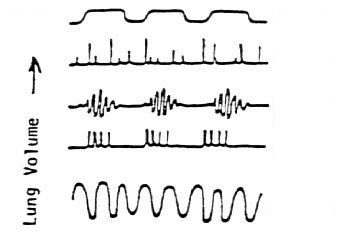
\includegraphics[width=0.48\textwidth]{./abnormalBreathingPatterns.jpg}
     \end{center}
    \caption{Elenco di pattern respiratori \cite{ABP}}
    \label{respirazioneAnormali}
\end{wrapfigure}



\paragraph{Apneosi.}
L'apneosi \`e uno schema di respirazione caratterizzato da profondi annaspamenti durante l'inspirazione, dopo una inspirazione avviene una lunga pausa seguita da un rilascio insufficiente di aria.
Notiamo che durante l'apneosi la pausa avviene dopo l'inspirazione e non dopo l'espirazione come nella sindrome da apnea ostruttiva.

\paragraph{Respiro agonico.}
Il respiro agonico \`e uno schema anormale di respirazione caratterizzato da boccheggiamento e da una riduzione estrema della frequenza degli atti respiratori fino al loro totale arresto. 
L'uso corretto del termine si deve restringere all'ultimo respiro prima della morte. 

\paragraph{Respiro di Cheyne Stokes.}
Il respiro di Cheyne Stokes \`e uno schema di respirazione anormale nel quale il respiro si fa da prima progressivamente pi\`u frequente e profondo, poi la frequenza respiratoria diminuisce gradualmente fino a portare ad una apnea. 
Lo schema si ripete e ogni ciclo di solito dura dai $30$ secondi ai $2$ minuti. 

\paragraph{Respiro di Kussmaul.}
Il respiro di Kussmaul \`e una forma di iperventilazione compensatoria. 
\`E caratterizzato da atti respiratosi molto lenti ed in particolare da una inspirazione profonda e rumorosa a cui segue una breve apnea, poi una espirazione breve e gemente e infine una pausa post-espiratoria decisamente prolungata.


